\documentclass[../notes.tex]{subfiles}

\pagestyle{main}
\renewcommand{\chaptermark}[1]{\markboth{\chaptername\ \thechapter\ (#1)}{}}
\setcounter{chapter}{2}

\begin{document}




\chapter{???}
\section{Lecture 5: Quantum Principles for Spectroscopy (Part 2)}
\begin{itemize}
    \item \marginnote{1/19:}Today: How \emph{light} interacts with molecules.
    \item Review of the classical vs. quantum resonance criterion (driven harmonic oscillator vs. matching energy difference between states).
    \item Reminder of spectroscopic notation: $E''$ (ground state) vs. $E'$ (excited state).
    \item Different types of transitions (electronic, vibrational, rotational) can be observed using different parts of the EM spectrum (UV/Vis, IR/Raman, FIR/\si{\micro wave}) as probes.
    \item What does light actually do?
    \begin{itemize}
        \item Quantum mechanically, it's coupling to the eigenstates of the system.
        \item Quantum eigenstates are stationary.
        \item Light couples two states, dragging them together and mathematically creating a superposition.
    \end{itemize}
    \item Example.
    \begin{figure}[h!]
        \centering
        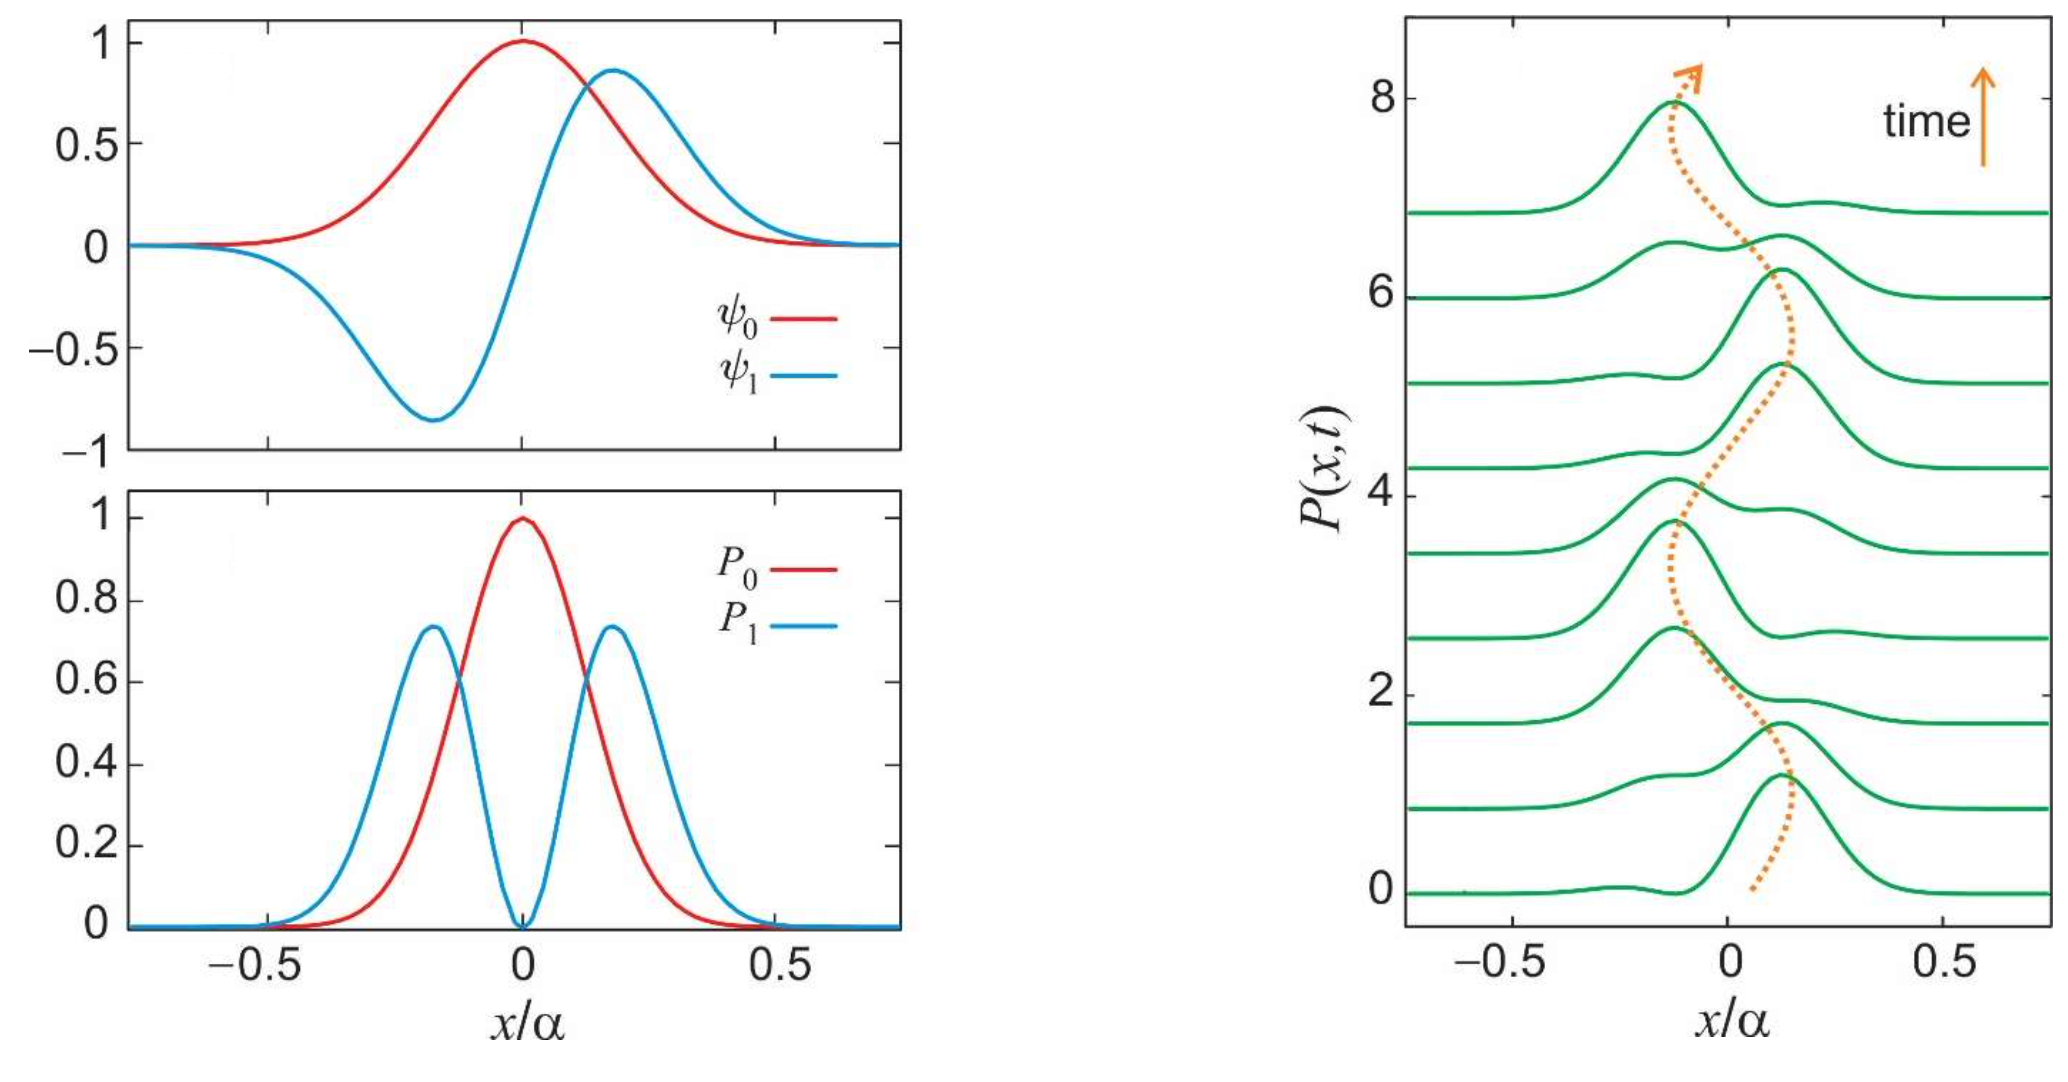
\includegraphics[width=0.7\linewidth]{lightCoupling.png}
        \caption{Light-induced coupling of quantum eigenstates.}
        \label{fig:lightCoupling}
    \end{figure}
    \begin{itemize}
        \item If we have two solutions to the particle in a box $\psi_0,\psi_1$ corresponding to the first and second energy levels, what light does is gives you a time-dependent wavefunction
        \begin{equation*}
            \psi(t) = c_0(t)\psi_0+c_1(t)\psi_1
        \end{equation*}
        \item The probability that the particle is in one state or the other oscillates: Since $c_n(t)=c_n\e[-iE_nt/\hbar]$,
        \begin{align*}
            P_1 &= |c_1(t)|^2 \approx \frac{\sin^2(E_1-E_0)t}{\hbar}&
            P_2 &= |c_0(t)|^2 \approx \frac{\cos^2(E_1-E_0)t}{\hbar}
        \end{align*}
    \end{itemize}
    \item Electronic degrees of freedom can be discussed in the same way.
    \begin{itemize}
        \item Light drives electrons back and forth (as per our classical molecule), but this time, we mathematically represent this change as a coupling of the $s$ orbital and the more elongated $p$ orbital.
    \end{itemize}
    \item Factors governing absorption strength.
    \begin{itemize}
        \item Beer's law.
        \item Two important factors.
        \begin{enumerate}
            \item Extinction coefficient.
            \item Concentration.
        \end{enumerate}
    \end{itemize}
    \item Quantum mechanically, absorption strength depends on state population.
    \begin{itemize}
        \item This is also a thermodynamic/statistical question.
        \item Thermal energy is distributed via the Boltzmann distribution.
        \item The probability of initially occupying an excited state increases with temperature.
    \end{itemize}
    \item Thermal energy distributes molecules through states with different rotational and vibrational states.
    \item Worry if $E_\text{rot}'',E_\text{vib}''\leq 2k_\text{B}T$.
    \item Populations at higher states will give rise to additional features in the absorption spectrum.
    \item Final states don't matter for us because $E_\text{final}\gg k_\text{B}T$.
    \begin{itemize}
        \item The only place where final energy matters is NMR because changes are so small; this is also why NMR is performed at cryogenic conditions.
    \end{itemize}
    \item Transition dipole moment.
    \begin{itemize}
        \item Classical (we need a change to grab onto) v. quantum (we take our transition dipole operator and square ite expected value) again.
    \end{itemize}
    \item Selection rules.
    \begin{itemize}
        \item Light can drive a molecule to go up or down one vibrational quantum. This is not strictly true because most oscillators are \emph{not} harmonic oscillators. Greater transitions are called \textbf{overtones}.
        \item Rotations: Same type of thing with $\Delta J=\pm 1$.
    \end{itemize}
\end{itemize}




\end{document}